\documentclass[review]{elsarticle}
\usepackage{hyperref,lineno}
\usepackage{xcolor}
\usepackage[utf8]{inputenc}
\modulolinenumbers[5]

\newcommand{\memo}[2]{\textcolor{#1}{#2}}
\newcommand{\maria}[1]{\memo{red}{#1\\}}
\newcommand{\revise}[1]{\memo{blue}{#1\\}}

%\journal{Journal of Archaeological Science}


\bibliographystyle{model2-names.bst}\biboptions{authoryear}


\begin{document}

\begin{frontmatter}


\begin{abstract}

The aim of this study is to detect the patterns of olive oil production that link amphora workshops and amphoric stamps. Roman provinces such as Baetica became important production and distribution centers during the Roman Empire. However, it remains under debate how this province was organized and whether it is possible to identify patterns in the olive oil market. 

CAMBIAR

Our case of study has been focused on the production processes located in Baetica province (currently Andalusia) from 1st to 3rd AD. In particular, we want to explore economic dynamics that include the production and distribution of olive oil trade. Amphoric stamps are used to identify the presence of different producer groups that might share similar stamps. To achieve this goal, we analyse a set of stamps from different workshops in Baetica province in order to detect a relation between the distribution of amphoric stamps and the economic structure in this province. Here we use methods borrowed from Ecology that allow us to identify if amphora workshops share similar amphoric stamps depending on the spatial distance. 

The analysis explores how quantitative approach provides a useful tool for the interpretation of the economic processes. Finally, results pretend to highlight the organization of Baetican olive oil production in the Roman Empire linked to the differences observed in the archaeological evidence.

\end{abstract}


\end{frontmatter}

\section{Introduction}


%primer párrafo más general---- especifico (¿dónde se ha aplicado?)
Material culture is one of the most frequent indicator of trade in the archaeological record. They allows us to highlight a part of mechanism of production and distribution of goods between different communities.  

%Roman trade has been an object of study in the last centuries. 


%This paper explore--- resumir en dos líneas el objeto de estudio y definir que ha sido usado para ello
This paper aims to highlight the production dynamics in relation to a specific area within Roman Empire. We want to detect the pattern of olive oil production that link amphora workshops and amphoric stamps used to mark them. We focus here on exploring the economic relation between stamps and amphora production centres. An ecology approach has been used to analyse the dispersion of stamps between amphora workshops. 

% hipotesis

% Debate
The discussion about the production processes in Baetican area due to the lack of written sources
In archaeology, this debate has been widely studied in the last centuries (CITAR). Despite this knowledge the application of new methodology to understand the Roman trade has allowed us to deal with the complexity of Roman Market combined with archaeological evidence \citep{orengo_seeds_2016,brughmans_roman_2016,coto-sarmiento_maria_bayesian_????}. Specifically, our work pretend to detect economic processes in a microescala focused in a commercial product from a specific province \citep{isaksen_network_2006}. 


%más específico--- olive oil

Roman province such as Baetica (currently Andalusia, south Spain) became important production centers of olive oil in the Roman Age. Olive oil was an important product during the Roman Empire used in almost all the aspect of daily life as cooking, hygiene or lightning \citep{mattingly_d.j._oil_1988}. 

The high demand of Roman provinces stimulated by the good condition of the Baetica lands allowed to develop a massive infrastructure of olive oil production. This product was distributed in large amount of amphorae along the province, mostly to supply the Roman Army and Italy \citep{blazquez_exportacion_1980}. 

The production and distribution of olive oil in this ancient province were growing exponentially during almost three centuries (cronologiaaa CITAR). As a results, hundred of amphora workshops were created to support this high demand. These workshops were located along the river Guadalquivir and its tributary Genil supplying from the riverine connectivity to the Mediterranean and Atlantic \citep{garcia_vargas_enrique_formal_2010}. 

The majority of olive oil amphorae produced in this province and shipped thought the provinces belong to Dressel 20 type \citep{dressel,martin-kilcher_romischen_1994}. This amphora is commonly associated with transportation of Baetican olive oil during the Roman Empire \citep{berni_millet_epigrafianforica_2008}. Most Dressel 20 were marked in stamps and \textit{tituli picti} and inked in graffities with different information but there is not a general consensus about the meaning of them \citep{rodriguez_baetican_1998}. Stamps are the most studied in this type of amphorae. There is evidence that stamps were used for almost three centuries. (economía oleica betica). Frequently, stamps were marked mainly in handles but rarely in rims and body \citep{millet_anforas_1998}. 
The information of the stamps is shown in different forms and letter content and it seems that there was not a unique criteria (CITAR). Stamps was mostly formed for a code of three letters. There letters can appear in a abbreviated form or complete and they are known as \textit{Tria Nomina} \citep{berni_millet_amphora_1996}. 
The meaning of the amphora stamps is still under debate. Some authors suggest that they were identified as the land-owners of the olive groves \citep{rodriguez_economioleicola_1977}. Other authors propose that stamp could be the owners of the making-amphorae workshop (CITAR) or even a production counting system \citep{berni_millet_epigrafianforica_2008}. In any case, the use of these stamps defined somehow the system of working in the workshops. 

%Hyphotesis
However, some challenges remain under discussion such as how this province was organized and whether it is possible to distinguish production patterns in the olive oil trade. Our questions will be focused on the distribution of amphoric stamps. Did they follow some distribution pattern? Did stamps share the same workshop? Neither written evidences have been found that it could explain the economic role of Baetica province in the Roman organization. On the other hand, archaeological evidence show a highly specialized production with a long activity in a this specific area with apparently few changes \citep{remesal_anforas_2004}. 

%hipotesis: si esto es así entonces es asá

Here, therefore, this study propose an approach to explore the effect of Baetican olive oil production by estimating of similarity index (COPIADO CAMBIAR). The assumption of this analysis is that closer workshops concentrate similar amphoric stamps in a specific area than the farthest workshops. By contrast, if we found similar amphoric stamps in different areas between workshops then the correlation between spatial distance would not be valued.  

%resumen del paper



%hablar de las tres áreas de producción: hispalis, corduba y astigi

%this paper aims to highlight the production dynamic in connection with the proximity between amphora workshops and stamps. 


\section{Material and Methods}

\subsection{Case study}

Our case study examines the relation between the distribution of amphoric stamps and the workshops. We studied a dataset of 3787 stamps collected from different amphora workshops in Baetica provice by CEIPAC database \citep{remesal_centro_2015} (see CEIPAC database). The workshops were situated in different locations in Baetica province, along the river Guadalquivir and its tributary Genil in order to detect similarities between stamps from workshops and spatial distance. 

However, approximately the 70 \% of stamps cannot be tested due to fragmentation or incomplete information. Consequently, we discard integrate the fragmented stamps in our dataset. We finally filter a total sample of 987 stamps composed by 131 different stamps from 81 workshops. 

The chronology in the workshops is widely diverse from the first to the third centuries AD (CITAR). However, some stamps show a more specific chronology while the majority of them display a large activity of production being difficult to specify an accurate chronology. A reason may be that most of them were partially excavated and only focused on archaeological surveys to collect the maximum stamps as possible (CITAR) 

%los sellos fueron marcados a partir del siglo II d.C (la economía oleícola bética Remesal) hablar de stams más concreto

%%\subsection{Jaccard distance}
%The dataset was analysed using a statistic method as Jaccard distance. This method allows to measure the dissimilarity by calculating the presence of sets (CITAR). In our case, Jaccard distance was used to compute the mutual presence of traits in the amphora stamps but it does not consider the number of absences. A comparison was done with the distance of the workshops to identify whether there was an association between stamps and spatial distance amongst workshops. 

\subsection{Quantifying the diversity Dissimilarity correlation}

%quizás habría que hablar también del filtrado de códigos que se hizo en python porque antes había 3783 stamps pero se filtró por el número de letras...

The approach proposed here is based on the idea of measuring the similarity between amphora workshops by quantifying similar stamps. A measure of dissimilarity has been chosen to analyse the dataset. We use the statistical technique Morisita-Horn index. The formula can be described as follows

(FORMULA Y DESCRIPCIÓN)


This method was performed to measure the overlap between different samples of sets \citep{morisita_measuring_1959, horn_measurement_1966}. In Ecology, it describes the dissimilarity between the system of two communities. 

Considering our dataset as non-uniform sample, this method provides a useful tool to handle large samples with different sizes and diversity \citep{wolda_similarity_1981}. Morisita-Horn index can be expressed considering 0 as total presence of similarity of stamps and 1 a totally dissimilarity between stamps. In our case, it will be calculated the number of times that one stamp appear in a amphora workshop. This method allows to bear in mind the similar number of times for each repeated stamp per workshop. 
%quizas ampliar con el método de xavielin

%hablar sobre Horn (Morisita)hablar sobre que el sample no estaba uniforme por eso usamos el morisita horn

\section{Results}

The analysis shows that amphoric stamps could not be correlated with spatial distance. 

The correlation coefficients range from a minimum to a maximum. The dendrogram shown in Fig. 2 \ref{dendro} was obtained with Morisita-Horn index. This dendrogram suggests that amphora workshops used different stamps for their prodution system. Accordingly only few closer workshops show a similarity on the stamps while most of them seem to display different stamps roles. 

\begin{figure}[htp]
	\centering
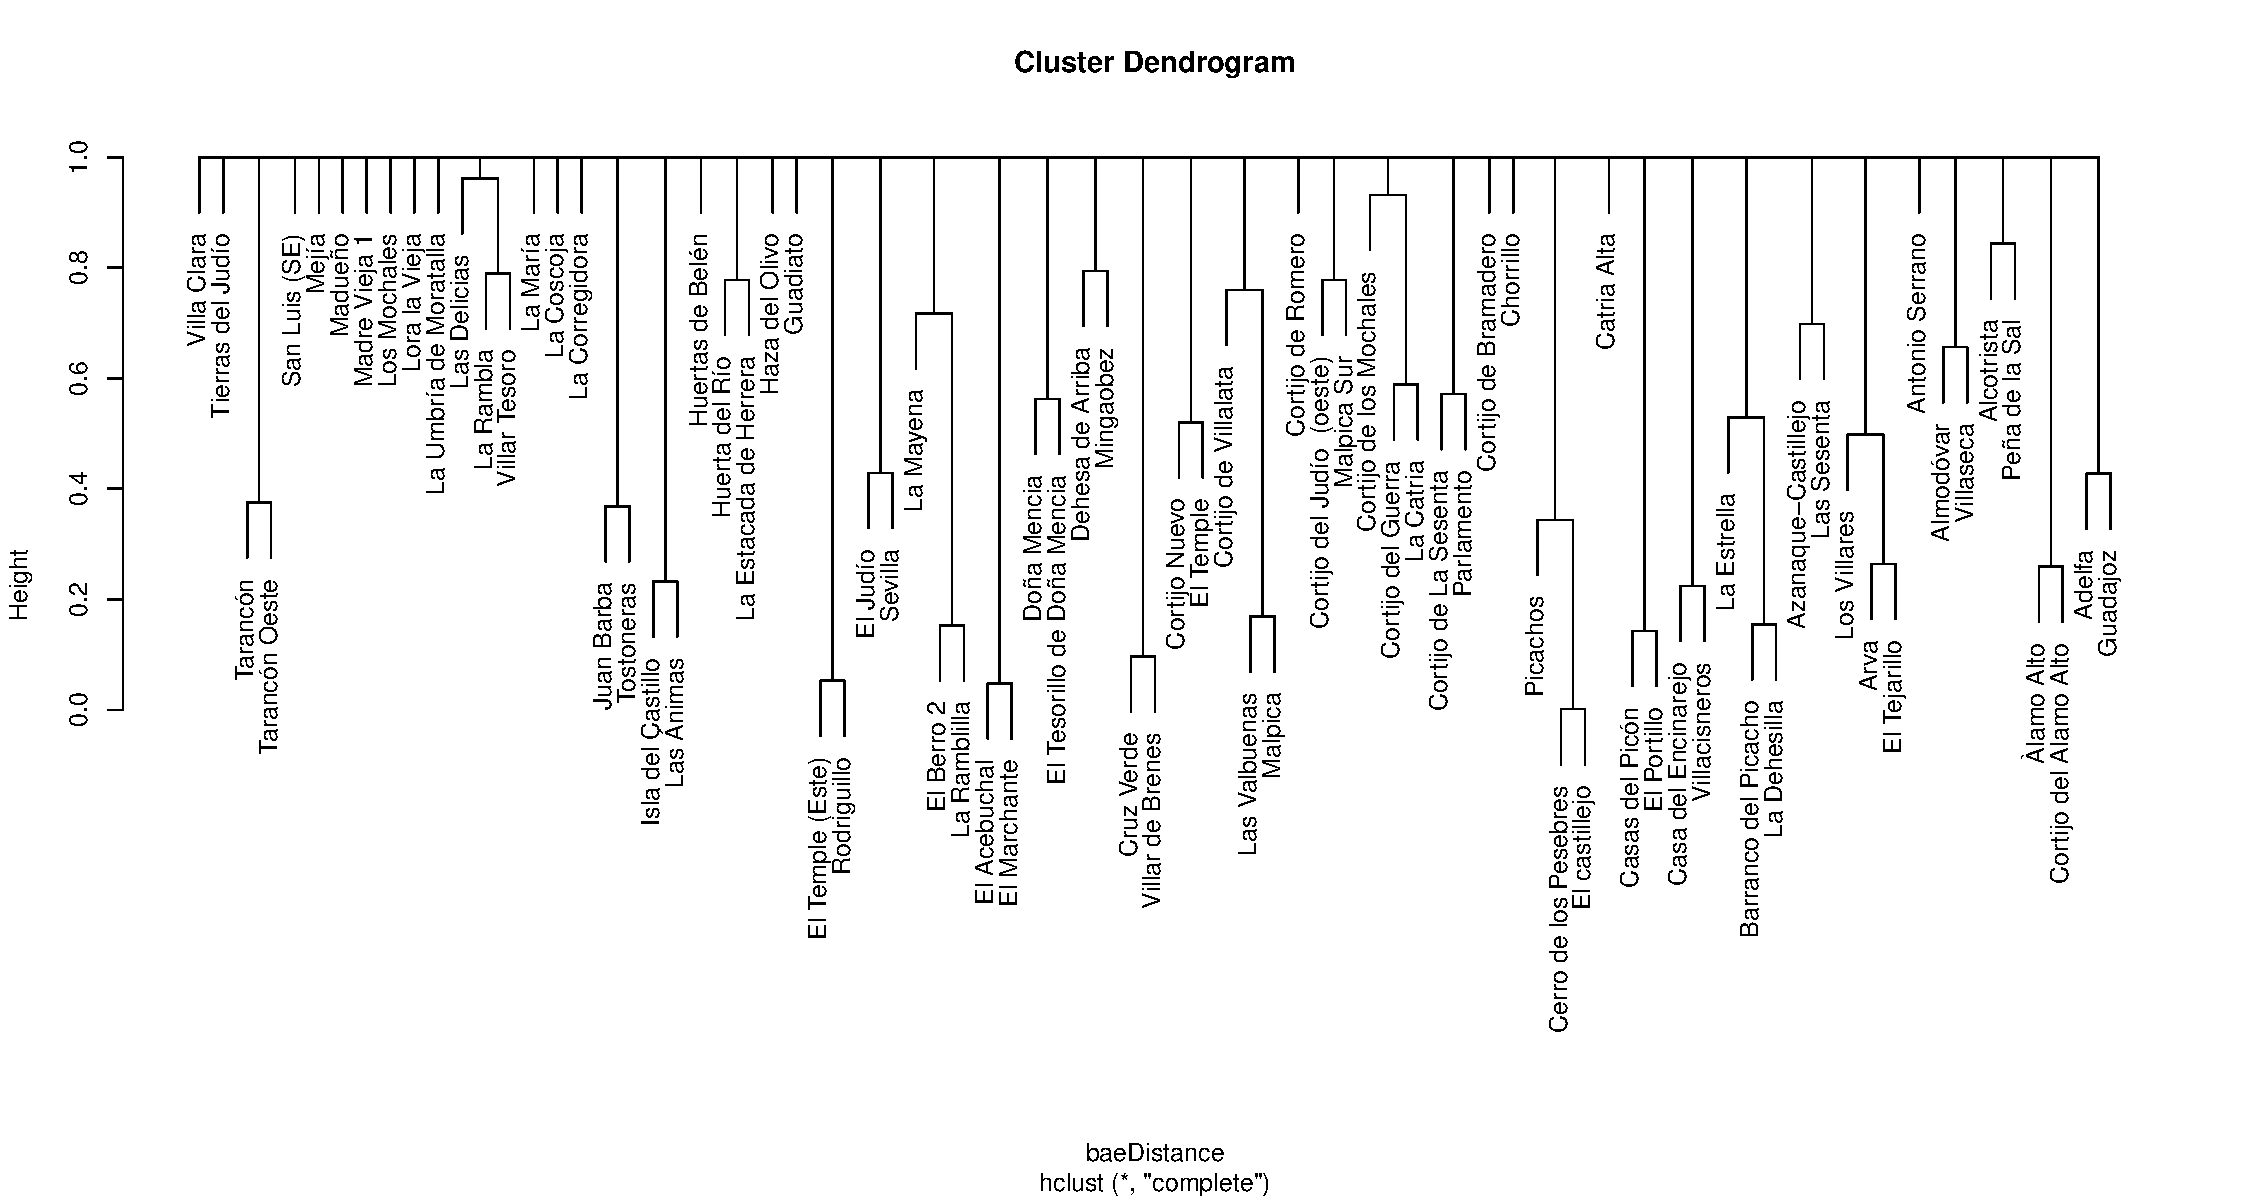
\includegraphics[width=\linewidth]{figs/dendro}
\caption{Dendrogram obtained by Morisita-Horn algorithm of different amphora workshops in Baetica area}
\label{dendro}
\end{figure} 


%%\subsection{Jaccard distance}

%Result of Jaccard distance can be The coefficients range from x to x.The dendrogram shown in Fig. Bla bla was obtained with the Jaccard distance measure. The dendrogram suggests 


\section{Discussion and Conclusion}

No strong relation between stamps and spatial distance have been detected in amphora workshops. Indeed, the analysis suggests that there is not connection between stamps and the same amphora workshops, excluding certain exceptions. Consequently the majority of stamps are located in different amphora workshops and only similar stamps between closer amphora workshops were found. In any case, our results show that most similar amphoric stamps were detected in closer workshops and not in other areas. These stamps tend to share the same area of production but there is not a general relation between groups of amphora workshops and area. 

The hypothesis about groups of amphora workshops sharing the same stamps seems not match with the results of analysis even though there are similar stamps in closer workshops. Rather the stamps detected in closer amphorae workshops seem not move from other farthest workshops. Additionally they could have been catalogued with different names by authors (METER PONSICH Y DRESSEL) in spite of belonging to the same place or being closer between each other. We also identify different stamps in other closer workshops. 
%los que aparecen cerca son porque están cerca o puede haber confusion entre talleres

By contrast, we have located different stamps in a same amphora workshop. Neither it seems that stamps were used to specify the quality or value of the product \citep{callender}. Probably our results could be interpreted due to several reason according to previous hypotheses. The use of these amphoric stamps could be exclusively running by the owner or families to distinguish the amphora workshop (CITAR). 

(aumentar)
On the other hand, it can be interpreted somehow a batch systematic organization to prepare and distribute the commodity considering that Dressel 20 type was not marked in several cases (CITAR)


it could be somehow a batch systematic organization to prepare and distribute the commodity, considering that Dressel 20 was not marked in several cases. This method was used of counting BLA BAL 

 

An any case, 

As summary, this method presented here provides a potential tool to understand mechanisms of production based on the similarity of artefacts. This method have identified differences in the case of the amphoric production within Roman Empire. Accordingly the results have highlighted to interpreter the complex economical processes based on  the archaeological evidence. 





%Dressel 20 marked in the 30-40\%

\section{Acknowledgements}

The research was funded by European Research Council Advanced Grant EPNet (340828). We are grateful to Simon Carrignon. 
All data has been analysed and conducted in R program version 3.2.4, using vegan package (citar) 


\section{References}

\bibliography{bibliotex}



\end{document}